\section{Augmentation of tLDGBAs and Synthesis Method}

We introduce an automaton augmented with binary vectors. The automaton can explicitly represent whether transitions in each accepting set occur at least once, and ensure transitions in each accepting set occur infinitely often.

Let $V = \{ (v_1, \ldots ,v_n)^T\ ;\ v_i \in \{ 0,1 \},\ i \in \{ 1, \ldots ,n \} \}$ be a set of binary-valued vectors, and let $\bm{1}$ and $\bm{0}$ be the $n$-dimentional vectors with all elements 1 and 0, respectively.
In order to augment a tLDBA $B_{\varphi}$, we introduce three functions $visitf:\delta \rightarrow V$, $reset:V \rightarrow V$, and $Max:V\times V \rightarrow V$ as follows.
For any $e \in \delta$, $visitf(e) = (v_1, \ldots ,v_n)^T$, where %$ v_i = 1 $ if $ e \in F_i $ and $ v_i=0 $ otherwise.
\begin{align}
 v_i =
  \left\{
  \begin{aligned}
    1 &   & &\text{if}\ e\in F_i, \\
    0 &   & &\text{otherwise}.
  \end{aligned}
  \right. \nonumber
\end{align}
For any $v \in V$, %$ reset(v) = \bm{0} $ if $ v = \bm{1} $ and $ reset(v) = v $ otherwise.
\begin{align}
  &reset(v) =
  \left\{
  \begin{aligned}
    \bm{0} &   & &\text{if}\  v = \bm{1},\\
    v &   & &\text{otherwise}.
  \end{aligned}
  \right. \nonumber
\end{align}
For any $v,u \in V$, $Max(v,u) = (l_1,\ldots ,l_n)^T$, where $l_i = max\{v_i, u_i\} $ for any $i\in \{1, \ldots ,n\}$.

Each vector $v$ is called a memory vector and represents which accepting sets have been visited. The function $visitf$ returns a binary vector whose $i$-th element is 1 if and only if a transition in the accepting set $F_i$ occurs. The function $reset$ returns the zero vector $\bm{0}$ if at least one transition in each accepting set has occurred after the latest reset. Otherwise, it returns the input vector without change.

\begin{definition}[Augmented Automata]
   For a tLDGBA $B_{\varphi} = (X,x_{init},\Sigma,\delta,\mathcal{F})$, its augmented automaton is a tLDGBA $\bar{B}_{\varphi}$ = $(\bar{X},\bar{x}_{init},\bar{\Sigma},\bar{\delta},\bar{\mathcal{F}})$, where $\bar{X} = X\times V$, $\bar{x}_{init} = (x_{init}, \bm{0})$, $\bar{\Sigma} = \Sigma$, $\bar{\delta}$ is defined as $\bar{\delta}$ = $\{ ((x,v), \bar{\sigma}, (x^{\prime},v^{\prime})) \in \bar{X} \times \bar{\Sigma} \times \bar{X}\ ;\ (x,\bar{\sigma},x^{\prime}) \in \delta,\ v^{\prime} = reset(Max(v,visitf((x,\bar{\sigma},x^{\prime})))) \}$, and $\mathcal{\bar{F}} = \{ \bar{F_1}, \ldots ,\bar{F_n} \}$ is defined as $\bar{F_i} = \{ ((x,v), \bar{\sigma}, (x^{\prime},v^{\prime})) \in \bar{\delta}\ ;\ (x, \sigma, x^{\prime}) \in F_i,\ v_i = 0 \}$ for each $ i \in \{1,...,n\}$.
   \label{augment_def}
\end{definition}

%It is obvious by Definition \ref{augment_def} that a tLDGBA and its augmented automaton accept the same language.
We denote by $\mathcal{L}(B)$ the accepted language of a tLDGBA $B$, namely the set of all infinite words accepted by $B$.

\begin{proposition}
  Let $ B = (X,x_{init},\Sigma,\delta,\mathcal{F}) $ and $ \bar{B} = (\bar{X},\bar{x}_{init},\bar{\Sigma},\bar{\delta},\bar{\mathcal{F}}) $ be an arbitrary tLDGBA and its augmentation, respectively.
Then, we have $ \mathcal{L}(B) = \mathcal{L}(\bar{B}) $.
\label{prop3-1}
\end{proposition}
The proof of Proopsition \ref{prop3-1} is shown in Appendix A.

The augmented tLDGBA $\bar{B}_{\varphi}$ keeps track of previous visits to the accepting sets of $B_{\varphi}$.
Intuitively,
% for an input word $w$,
along a run of $\bar{B}_\varphi$,
a memory vector $v$ is reset to $\bm{0}$ when at least one transition in each accepting set of the original tLDGBA $B_{\varphi}$ has occurred.
% along the corresponding run of $B_{\varphi}$.

For example, shown in Figs.\ \ref{automaton} and \ref{automaton_aug} are a tLDGBA and its augmented automaton, respectively, associated with the following LTL formula.
\begin{align}
  \varphi = \text{{\bf GF}}a \land \text{{\bf GF}}b \land \text{{\bf G}}\neg c.
  \label{ltl}
\end{align}
The acceptance condition ${\mathcal F}$ of the tLDGBA is given by ${\mathcal F} = \{ F_1,F_2 \}$, where $F_1=\{ (x_0, \{ a \}, x_0),\ (x_0, \{ a,b \}, x_0) \}$ and $F_2 = \{ (x_0, \{ b \}, x_0),\ (x_0, \{ a,b \}, x_0) \}$.
Practically, states in a strongly connected component that contains no accepting transitions can be merged as shown in Fig.\ \ref{automaton_aug}.

\begin{figure}[htbp]
   \centering
%   \vspace{2mm}
%   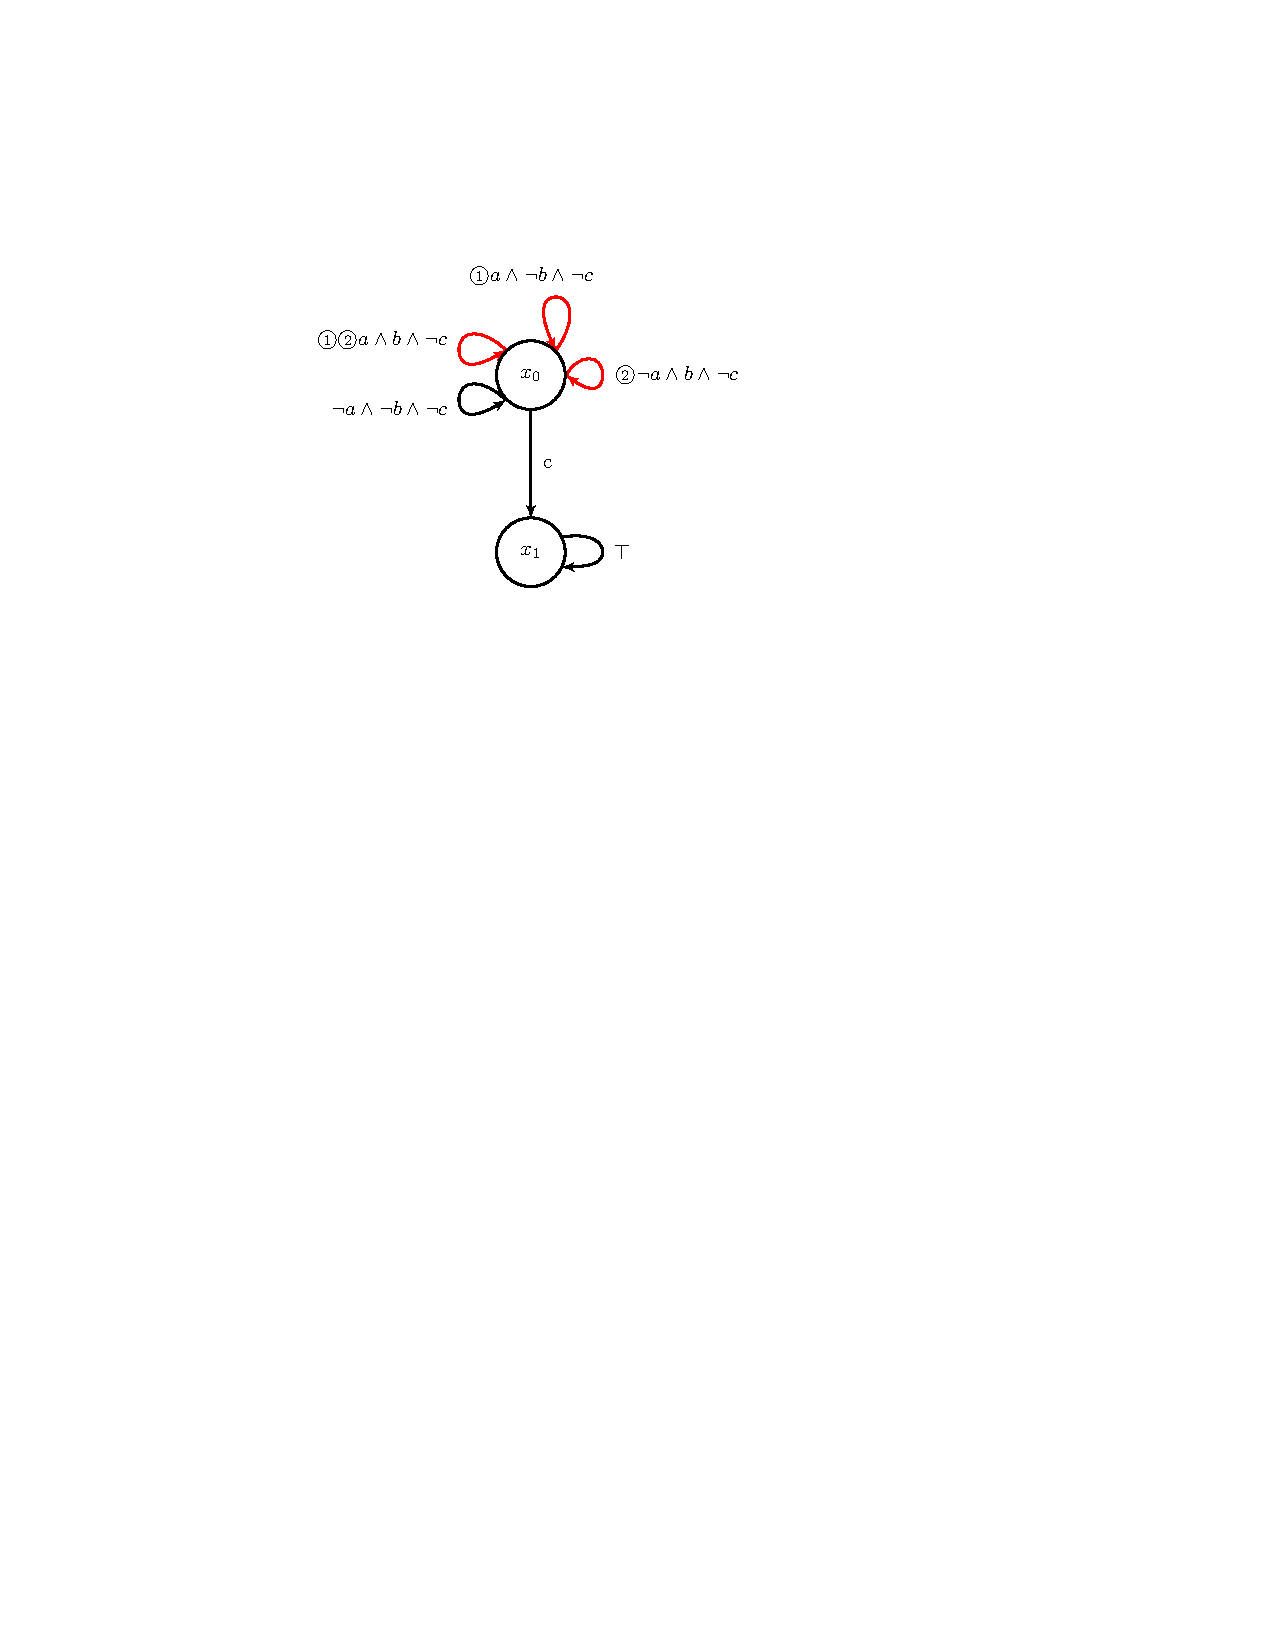
\includegraphics[bb=140 498 368 682,width=5cm]{automaton1.pdf}
   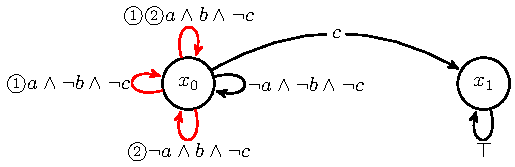
\includegraphics[bb=0 0 247 80,scale=0.75]{ldgba_original.pdf}
   \caption{The tLDGBA recognizing the LTL formula $\text{{\bf GF}}a \wedge \text{{\bf GF}}b \wedge \text{{\bf G}}\neg c$, where the initial state is $x_0$. Red arcs are accepting transitions that are numbered in accordance with the accepting sets they belong to.}
   % e.g., \textcircled{\scriptsize 1}$a \land \neg b \land \neg c$ means the transition labeled by it belongs to the accepting set $F_1$.}
   \label{automaton}
\end{figure}
\begin{figure}[htbp]
   \centering
%   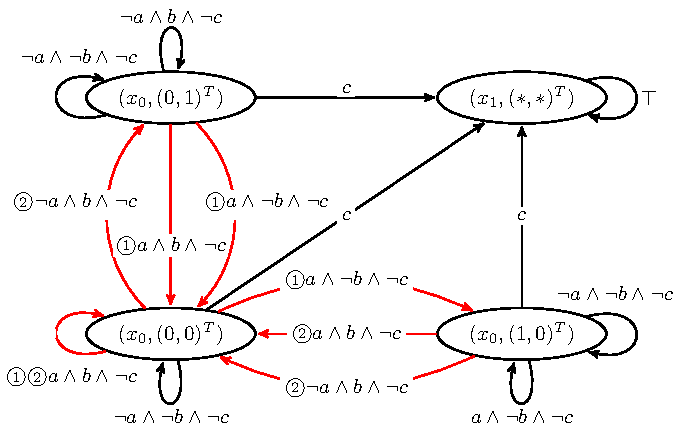
\includegraphics[bb=0 0 374 207,height=4cm, width=7cm]{ldgba.pdf}
   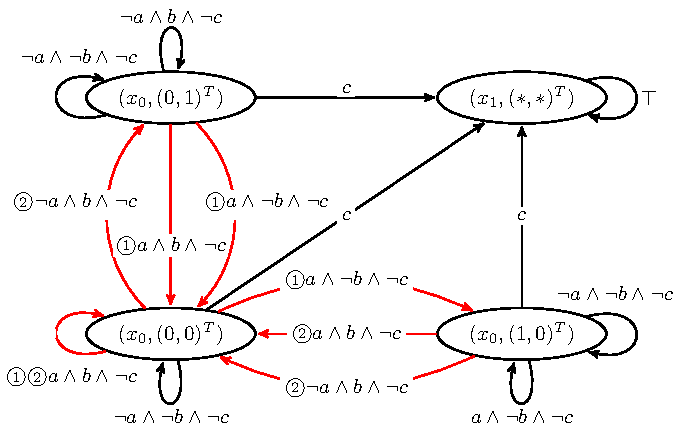
\includegraphics[bb=0 0 326 207,scale=0.75]{ldgba.pdf}
   \caption{The augmented automaton for the tLDGBA in Fig.~\ref{automaton} recognizing the LTL formula $\text{{\bf GF}}a \wedge \text{{\bf GF}}b \wedge \text{{\bf G}}\neg c$, where the initial state is $(x_0, (0,0)^T )$. Red arcs are accepting transitions that are numbered in accordance with the accepting sets they belong to. All states corresponding to $x_1$ are merged into $(x_1, (*,*)^T )$.}
   \label{automaton_aug}
\end{figure}

We modify the standard definition of a product MDP to deal with $\varepsilon$-transitions in the augmented automaton.
\begin{definition}[Product MDPs]
  Given an augmented tLDGBA $\bar{B}_{\varphi}$ and an MDP $M$, a tuple $M \otimes \bar{B}_{\varphi} = M^{\otimes} = (S^{\otimes}, A^{\otimes},s_{init}^{\otimes}, P^{\otimes}, \delta^{\otimes},$ $ {\mathcal F}^{\otimes})$ is a product MDP, where
  $S^{\otimes} = S \times \bar{X}$ is the finite set of states;
  $A^{\otimes}$  is the finite set of actions such that $A^{\otimes}=A \cup \{ \varepsilon_{\bar{x}^{\prime}} ; \exists \bar{x}^{\prime}\! \in \! X \text{ s.t. } (\bar{x},\varepsilon,\bar{x}^{\prime}) \in \bar{\delta} \}$, where $\varepsilon_{\bar{x}^{\prime}}$ is the action for the $\varepsilon$-transition to the state $\bar{x}^{\prime}\! \in\! \bar{X}$;
  $s_{init}^{\otimes} = (s_{init},\bar{x}_{init})$ is the initial state; $P^{\otimes} : S^{\otimes} \times S^{\otimes} \times A^{\otimes} \rightarrow [0,1]$ is the transition probability function defined as
%   $P^{\otimes}(s^{\otimes \prime} | s^{\otimes}, a) = P(s^{\prime} | s, a)$ if $ (\bar{x}, L((s,a,s^{\prime})), \bar{x}^{\prime}) \in \bar{\delta}$ and $ a \in \mathcal{A}(s)$, $P^{\otimes}(s^{\otimes \prime} | s^{\otimes}, a) = 1$ if $s\!=\!s^{\prime}, (\bar{x}, \varepsilon, \bar{x}^{\prime})\! \in \! \bar{\delta},$ and $ a=\varepsilon_{x^{\prime}}$, otherwise $P^{\otimes}(s^{\otimes \prime} | s^{\otimes}, a) = 0$
%   \begin{comment}
  \begin{align*}
    &P^{\otimes}(s^{\otimes \prime} | s^{\otimes}, a) \\ &=
    \left\{
    \begin{aligned}
      &P(s^{\prime} | s, a) &   &\text{if}\  (\bar{x}, L((s,a,s^{\prime})), \bar{x}^{\prime}) \in \bar{\delta}, a \in \mathcal{A}(s)\\
      &1 &   &\text{if}\ s=s^{\prime}, (\bar{x}, \varepsilon, \bar{x}^{\prime}) \in  \bar{\delta}, a=\varepsilon_{\bar{x}^{\prime}},\\
      &0 &   &\text{otherwise} ,
    \end{aligned}
    \right. \nonumber
  \end{align*}
% \end{comment}
  where $s^{\otimes}=(s,(x,v))$ and $s^{\otimes \prime}=(s^{\prime},(x^{\prime},v^{\prime}))$;
  $\delta^{\otimes} = \{ (s^{\otimes}, a, s^{\otimes \prime})\in S^{\otimes} \times A^{\otimes} \times S^{\otimes} ; P^{\otimes}(s^{\otimes \prime} | s^{\otimes}, a) > 0 \}$ is the set of transitions;
  and ${\mathcal F}^{\otimes} = \{ \bar{F}^{\otimes}_1, \ldots ,\bar{F}^{\otimes}_n \}$ is the acceptance condition, where $\bar{F}^{\otimes}_i = \{ ((s,\bar{x}), a, (s^{\prime}, \bar{x}^{\prime})) \in \delta^{\otimes} ; (\bar{x}, L(s,a,s^{\prime}), \bar{x}^{\prime}) \in \bar{F}_i \}$ for each $ i \in \{ 1, \ldots ,n \}$.
  \begin{comment}
   We have to modify the definition of product MDP to deal with $\varepsilon$-transitions in the original tLDBA $B_{\varphi}$. First, for all $\varepsilon$-transition from $x \in X$ to $x^{\prime} \in X$ of $B_{\varphi}$, we add the $\varepsilon_{x^{\prime}}$-action into the product MDP, namely $\mathcal{A}^{\otimes}(s^{\otimes}) = \mathcal{A}^{\otimes}(s^{\otimes}) \cup \{ \varepsilon_{x^{\prime}} ; s^{\otimes} = (s,(x,v)),\ s^{\otimes \prime} = (s,(x^{\prime}, v)),\ x,x^{\prime} \in X \}$. Second, the transition probability associated with the $\varepsilon_{x^{\prime}}$-action is defined as
  \begin{align}
    P^{\otimes}(s^{\otimes \prime} | s^{\otimes}, a) =
    \left\{
    \begin{aligned}
      &1 &   &\text{if}\ (s\!=\!s^{\prime})\! \land\! (v\!=\!v^{\prime})\! \land\! (x, \varepsilon_{x^{\prime}}, x^{\prime})\! \in \! \bar{\delta},\\
      &0 &   &\text{otherwise} ,
    \end{aligned}
    \right. \nonumber
  \end{align}
  where $s^{\otimes}=(s,(x,v))$ and $s^{\otimes}=(s^{\prime},(x^{\prime},v^{\prime}))$.
\end{comment}

\label{def9}
\end{definition}

\begin{definition}[Reward assignments]
  The reward function $\mathcal{R} :S^{\otimes} \times A^{\otimes} \times S^{\otimes} \rightarrow {\mathbb R}_{\geq 0}$ is defined as
  \begin{align}
    \mathcal{R}(s^{\otimes}, a, s^{\otimes \prime}) =
    \left\{
    \begin{aligned}
      &r_p \  \text{if}\ \exists i \in \! \{ 1, \ldots ,n \},\ (s^{\otimes}, a, s^{\otimes \prime}) \in \bar{F}^{\otimes}_i \!,\\
      &0   \ \ \text{otherwise},
    \end{aligned}
    \right. \nonumber
  \end{align}
  where $r_p$ is a positive value.
  \label{def10}
\end{definition}

%The reward assignments are based on the acceptance conditions of the product MDP.
Under the product MDP $M^{\otimes}$ and the reward function $\mathcal{R}$, which is based on the acceptance condition of $ M^\otimes $, we show that if there exists a positional policy $\pi$ satisfying the LTL specification $\varphi$, maximizing the expected discounted reward produces a policy satisfying $\varphi$.

For a Markov chain $MC^{\otimes}_{\pi}$ induced by a product MDP $M^{\otimes}$ with a positional policy $\pi$, let $S^{\otimes}_{\pi}= T^{\otimes}_{\pi} \sqcup R^{\otimes 1}_{\pi} \sqcup \ldots \sqcup R^{\otimes h}_{\pi}$ be the set of states in $MC^{\otimes}_{\pi}$, where $T^{\otimes}_{\pi}$ is the set of transient states and $R^{\otimes i}_{\pi}$ is the recurrent class for each $i \in \{ 1, \ldots ,h \}$, and let $R(MC^{\otimes}_{\pi})$ be the set of all recurrent classes in $MC^{\otimes}_{\pi}$. Let $\delta^{\otimes}_{\pi,i}$ be the set of transtions in a recurrent class $R^{\otimes i}_{\pi}$, namely $\delta^{\otimes}_{\pi,i} = \{ (s^{\otimes},a,s^{\otimes \prime}) \in \delta^{\otimes} ; s^{\otimes} \in R^{\otimes i}_{\pi},\ P^{\otimes}(s^{\otimes \prime}|s^{\otimes},a) > 0 \}$, and let $P^{\otimes}_{\pi}$ : $S^{\otimes}_{\pi} \times S^{\otimes}_{\pi} \rightarrow [0,1]$ be the transition probability under $\pi$.

\begin{lemma}
  For any policy $\pi$ and any recurrent class $R^{\otimes i}_{\pi}$ in the Markov chain $MC^{\otimes}_{\pi}$,
  $MC^{\otimes}_{\pi}$ satisfies one of the following conditions.
  \vspace{2mm}
  \begin{enumerate}
    \item $\delta^{\otimes}_{\pi,i} \cap \bar{F}^{\otimes}_j \neq \emptyset\ $, $ \forall j \in \{ 1, \ldots ,n \}$,
    \item $\delta^{\otimes}_{\pi,i} \cap \bar{F}^{\otimes}_j = \emptyset\ $, $ \forall j \in \{ 1, \ldots ,n \}$.
  \end{enumerate}
  \label{lemma3-1}
\end{lemma}
The proof of Lemma \ref{lemma3-1} is shown in Appendix A.

Lemma \ref{lemma3-1} implies that for an LTL formula $\varphi$ if a path $\rho$ under a policy $\pi$ does not satisfy $\varphi$, then the agent obtains no reward in recurrent classes; otherwise there exists at least one recurrent class where the agent obtains rewards infinitely often.

\begin{theorem}
  Let $M^{\otimes}$ be the product MDP corresponding to an MDP $M$ and an LTL formula $\varphi$. If there exists a positional policy satisfying $\varphi$, then there exists a discount factor $\gamma^{\ast}$ such that any algorithm that maximizes the expected reward with $\gamma > \gamma^{\ast}$ will find a positional policy satisfying $\varphi$.
  \label{theorem3-1}
\end{theorem}
The proof of Theorem \ref{theorem3-1} is shown in Appendix A.

%\begin{theorem}
%  Let $M^{\otimes}$ be the product MDP corresponding to an MDP $M$ and an LTL formula $\varphi$. If there exists a positional policy $\pi$ such that $Pr^M_{\pi}(\rho_{init} \models \varphi) = 1$, then there exists a discount factor $\gamma^{\ast}$ such that any algorithm that maximizes the expected reward with $\gamma > \gamma^{\ast}$ will find a positional policy $\pi^{\prime}$ such that $Pr^M_{\pi^{\prime}}(\rho_{init} \models \varphi) = 1$.
%  \label{theorem3-2}
%\end{theorem}

We show the overall procedure of our proposed method in Algorithm \ref{syn_pol}. We employ Q-learning in Algorithm \ref{syn_pol}, but any algorithms maximizing the expected discounted reward can be applied to our proposed method.
\begin{algorithm}
 \caption{RL-based synthesis of control policy on the MDP with the augmented tLDBA.}
 \begin{algorithmic}[1]
 \renewcommand{\algorithmicrequire}{\textbf{Input:}}
 \renewcommand{\algorithmicensure}{\textbf{Output:}}
 \REQUIRE LTL formula $\varphi$ and MDP $M$
 \ENSURE  Optimal policy $\pi^{\ast}$ on the product MDP $M^{\otimes}$
 \STATE Translate $\varphi$ into tLDBA $B_{\varphi}$.
  \STATE Augment $B_{\varphi}$ to $\bar{B}_{\varphi}$.
  \STATE Construct the product MDP $M^{\otimes}$ of $M$ and $\bar{B}_{\varphi}$.
  \STATE Initialize $Q:S^{\otimes} \times A^{\otimes} \rightarrow \mathbb{R}_{\geq 0}$.
  \STATE Initialize episode length $T$.
  \WHILE {$Q$ is not converged}
  \STATE $s^{\otimes} \leftarrow (s_{init},(x_{init},\bm{0}))$.
  \FOR {$t = 1$ to $T$}
  \STATE Choose the action $a$ by a policy $\pi$.
  \STATE Observe the next state $s^{\otimes \prime}$.
  \STATE $Q(s^{\otimes},a) \leftarrow Q(s^{\otimes},a) + \alpha \{ \mathcal{R}(s^{\otimes},a,s^{\otimes \prime}) + \gamma \max_{a^{\prime}}Q(s^{\otimes \prime},a^{\prime}) - Q(s^{\otimes},a) \}$
  \STATE $s^{\otimes} \leftarrow s^{\otimes \prime}$
  \ENDFOR
  \ENDWHILE
 \end{algorithmic}
 \label{syn_pol}
\end{algorithm}

\section{Example}

\begin{figure}[tbp]
    \centering
    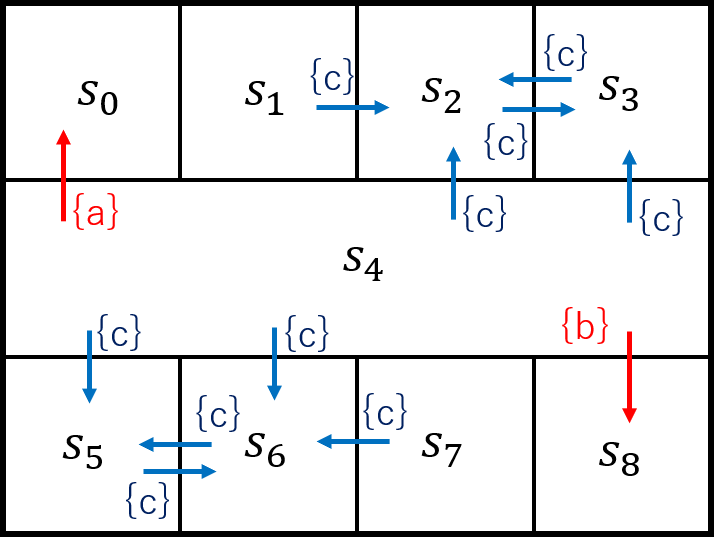
\includegraphics[bb=0 0 377 290,height=3.5cm,width=5cm]{MDP_corridor.png}
%    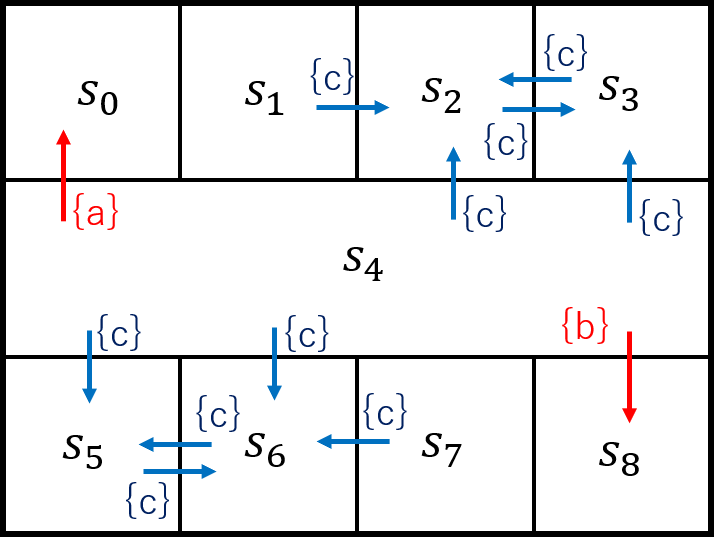
\includegraphics[height=4cm, width=6cm]{MDP_corridor.png}
    \caption{The environment consisting of eight rooms and one corridor. Red arcs are the transitions that we want to occur infinitely often, while blue arcs are the transitions that we never want to occur. $s_7$ is the initial state.}
    \label{Grid1}
\end{figure}

\begin{comment}
\begin{figure}[htbp]
   \centering
   \vspace{2mm}
%   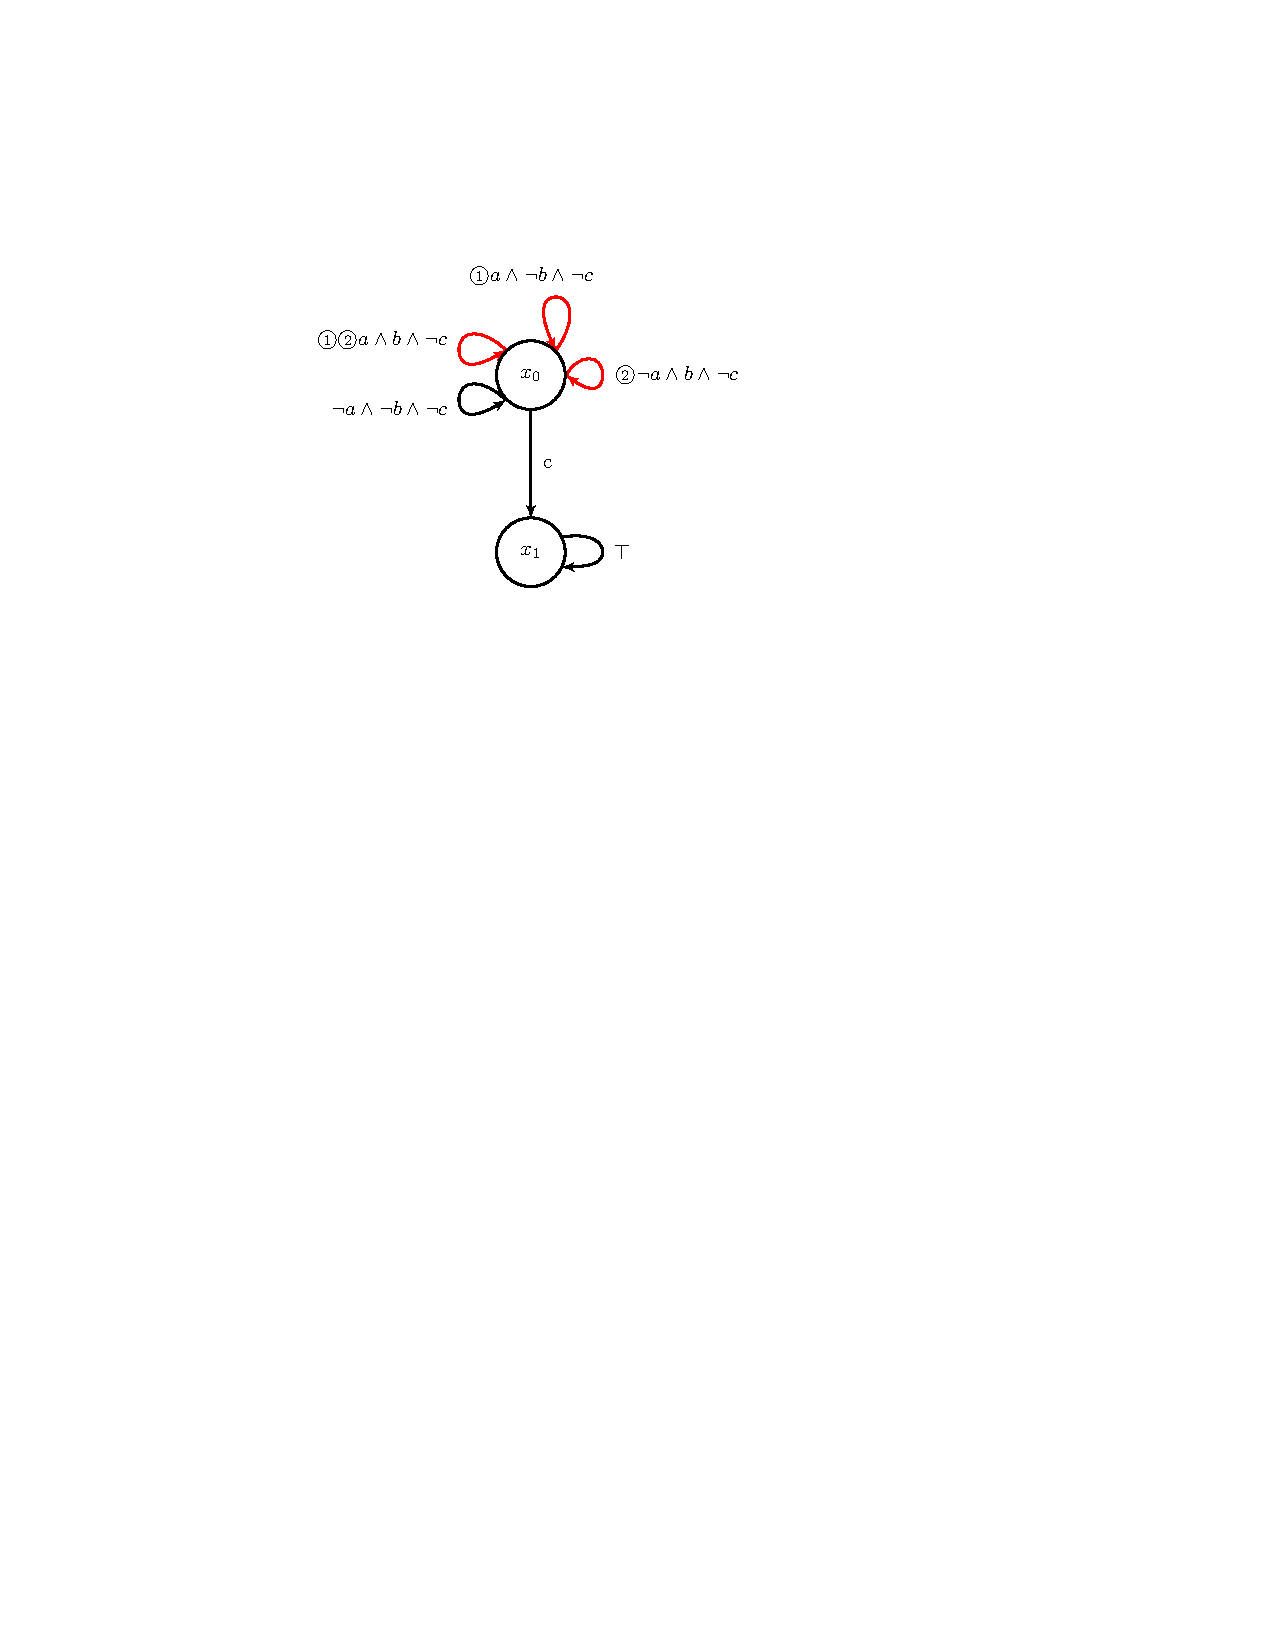
\includegraphics[bb=140 498 368 682,width=5cm]{automaton1.pdf}
   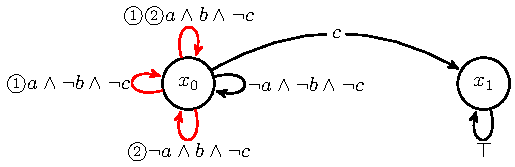
\includegraphics[bb=0 0 247 80,scale=0.65]{ldgba_original.pdf}
   \caption{The tLDGBA recognizing the LTL formula $\text{{\bf GF}}a \wedge \text{{\bf GF}}b \wedge \text{{\bf G}}\neg c$, where the initial state is $x_0$. Red arcs are accepting transitions that are numbered in accordance with the accepting sets they belong to.}
   % e.g., \textcircled{\scriptsize 1}$a \land \neg b \land \neg c$ means the transition labeled by it belongs to the accepting set $F_1$.}
   \label{automaton}
\end{figure}

\begin{figure}[htbp]
   \centering
%   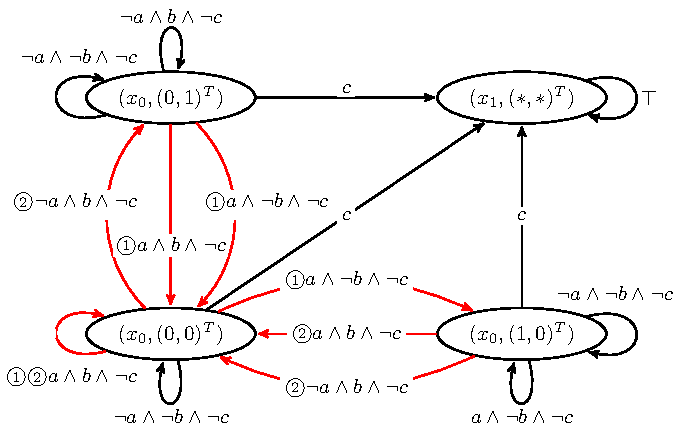
\includegraphics[bb=0 0 374 207,height=4cm, width=7cm]{ldgba.pdf}
   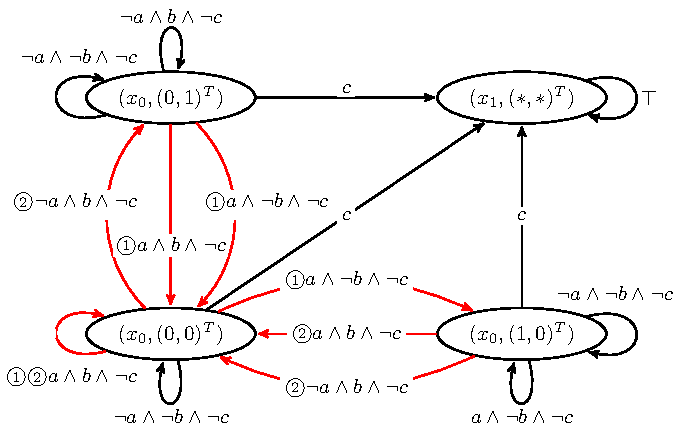
\includegraphics[bb=0 0 374 207,scale=0.6]{ldgba.pdf}
   \caption{The augmented automaton for the tLDGBA in Fig.~\ref{automaton} recognizing the LTL formula $\text{{\bf GF}}a \wedge \text{{\bf GF}}b \wedge \text{{\bf G}}\neg c$, where the initial state is $(x_0, (0,0)^T )$. Red arcs are accepting transitions that are numbered in accordance with the accepting sets they belong to. All states corresponding to $x_1$ are merged into $(x_1, (*,*)^T )$.}
   \label{automaton_aug}
\end{figure}
\end{comment}

In this section,
we apply the proposed method to a path planning problem of a robot in an environment consisting of eight rooms and one corridor as shown in Fig.\ \ref{Grid1}. The state $s_7$ is the initial state and the action space is specified with $\mathcal{A}(s) = \{ Right, Left, Up, Down \}$ for any state $s \neq s_4$ and $\mathcal{A}(s_4) = \{ to\_s_0, to\_s_1, to\_s_2, to\_s_3, to\_s_5, $ $to\_s_6, to\_s_7, to\_s_8 \}$, where $to\_s_i$ means attempting to go to the state $s_i$ for $i \in \{0,\ 1,\ 2,\ 3,\ 5,\ 6,\ 7,\ 8 \}$. The robot moves in the intended direction with probability 0.9 and it stays in the same state with probability 0.1 if it is in the state $s_4$. In the states other than $s_4$, it moves in the intended direction with probability 0.9 and it moves in the opposite direction to that it intended to go with probability 0.1. If the robot tries to go to outside the environment, it stays in the same state. The labeling function is as follows.
\begin{align*}
      & L((s, act, s^{\prime})) =
      \left\{
      \begin{aligned}
        & \{ c \} &  & \text{if }s^{\prime} = s_i,\ i \in \{ 2,3,5,6 \}, \nonumber \\
        & \{ a \} &  & \text{if }(s,act,s^{\prime})=(s_4,to\_s_0,s_0), \nonumber \\
        & \{ b \} &  & \text{if }(s,act,s^{\prime})=(s_4,to\_s_8, s_8), \nonumber \\
        & \emptyset &  & \text{otherwise}.
      \end{aligned}
      \right.
    \end{align*}

In the example, the robot tries to take two transitions that we want to occur infinitely often, represented by arcs labeled by \{$a$\} and \{$b$\}, while avoiding unsafe transitions represented by the arcs labeled by \{{\it c}\}. This is formally specified by the LTL formula given by (\ref{ltl}).
The LTL formula requires the robot to keep on entering the two rooms $s_0$ and $s_8$ from the corridor $s_4$ regardless of the order of entries, while avoiding entering the four rooms $s_2$, $s_3$, $s_5$, and $s_6$.
% They have two accepting sets.
%We use Owl \cite{Owl} to obtain the tLDBA corresponding to the LTL formula.
The tLDGBA $B_{\varphi} = (X, x_{init},\Sigma,\delta,\mathcal{F})$ and its augmented automaton $\bar{B}_{\varphi} = (\bar{X},\bar{x}_{init},\bar{\Sigma},\bar{\delta},\bar{\mathcal{F}})$ are shown in Figs.\ \ref{automaton} and \ref{automaton_aug}, respectively.

Through the above scenario,
we compare our approach with 1) a case where we first convert the tLDGBA into a tLDBA, for which the augmentation makes no change, and thus a reward function in Definition \ref{def10} is based on a single accepting set; and
2) the method using a reward function based on the accepting frontier function \cite{HAK2019,HKAKPL2019}.
% In the method using tLDBA, the reward function is defined like Definition \ref{def10}, namely it is based on the one accepting set of the corresponding product MDP.
For the three methods, we use Q-learning\footnote{We employ Q-learning here but any algorithm that maximizes the discounted expected reward can be applied to our proposed method.} with $\varepsilon$-greedy policy and gradually reduce $\varepsilon$ to 0 to learn an optimal policy asymptotically.
We set the positive reward $r_p = 2$, the epsilon greedy parameter $ \varepsilon = \frac{0.95}{n_t(s^{\otimes})}$, where $n_t(s^{\otimes})$ is the number of visits to state $s^{\otimes}$ within $t$ time steps \cite{Singh1998}, and the discount factor $\gamma = 0.95$. The learning rate $\alpha$ varies in accordance with {\it the Robbins-Monro condition}. We train the agent in 10000 iterations and 1000 episodes for 20 learning sessions.

\begin{figure}[tbp]
 \centering
 \begin{tabular}{c}
  \begin{minipage}{0.5\hsize}
     \centering
%     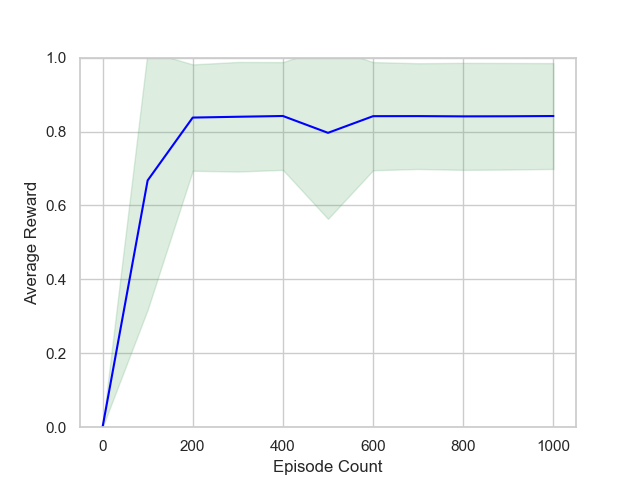
\includegraphics[width=4.5cm]{ep_1000_it_10000_MDP3_gamma_095_re2_ini22_nts_c095_20times.png}
     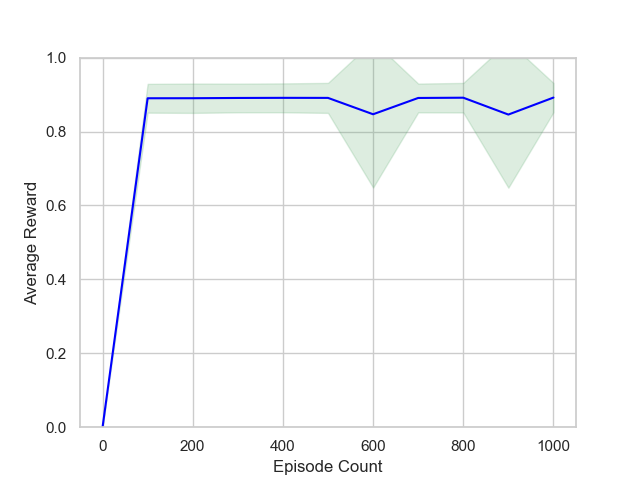
\includegraphics[bb=0 0 461 346, height = 3.3cm, width=4.2cm]{ep_1000_it_10000_MDP3_gamma_095_re2_ini22_nts_c095_20times_no3.png}
 \end{minipage}

 \begin{minipage}{0.5\hsize}
   \centering
%   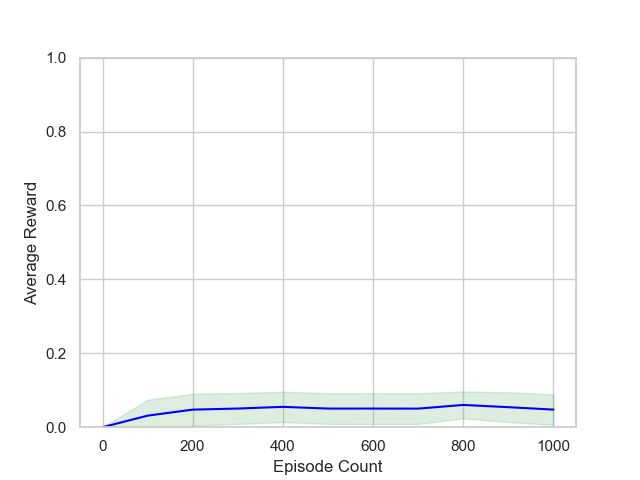
\includegraphics[width=4.5cm]{ep_1000_it_10000_MDP3_gamma_095_nts_c095_abate_20times.png}
   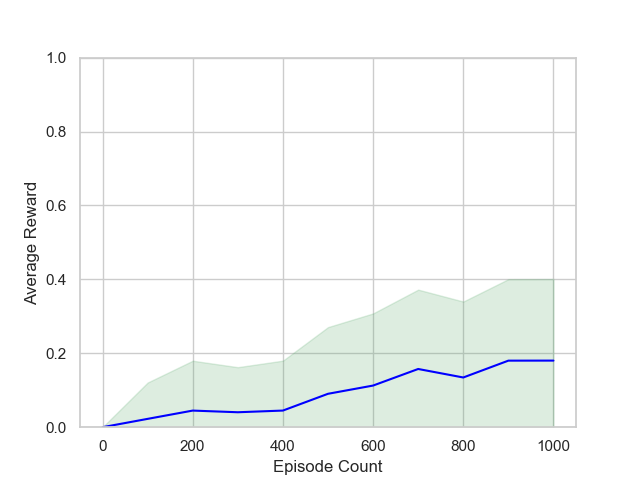
\includegraphics[bb=0 0 461 346, height = 3.3cm, width=4.2cm]{tex_resubmit/ep_1000_it_10000_MDP3_gamma_095_nts_c095_ldba_20times_no4.png}
 \end{minipage}
\end{tabular}
 \caption{The mean of average reward in each episode for 20 learning sessions obtained from our proposed method (left) and the method using tLDBA (right). They are plotted per 100 episodes and the green areas represent the range of standard deviations. }
 \label{result}
\end{figure}

\begin{figure}[tbp]
	\centering
	\begin{tabular}{c}

		\begin{minipage}{0.499\hsize}
		\centering
			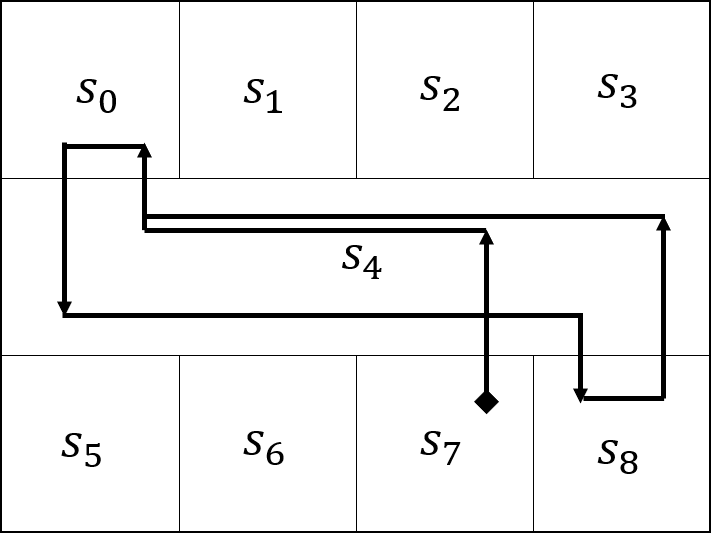
\includegraphics[bb=0 0 341 256, height = 2.7cm,
			width=3.5cm]{proposed_policy.png}
		\end{minipage}

		\begin{minipage}{0.499\hsize}
			\centering
			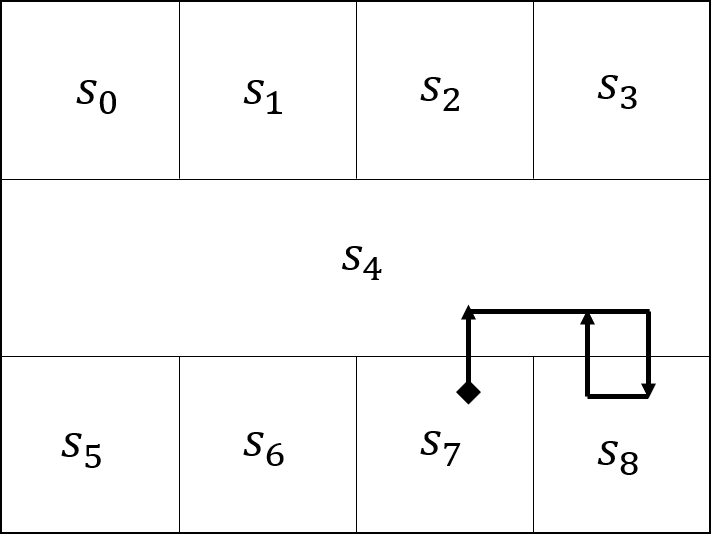
\includegraphics[bb=0 0 341 257, height = 2.7cm,
			width=3.5cm]{Abate_policy.png}
		\end{minipage}
	\end{tabular}

	\caption{The optimal policy obtained from our proposed method (left) and the method in \cite{HAK2019, HKAKPL2019} (right).}
	\label{optimal}
\end{figure}

%We conduct the same example with their method using the tLDGBA instead.
\subsection*{Results}
\textit{1) }
Fig.\ \ref{result} shows the average rewards obtained by our proposed method and the case using a tLDBA $B^{\prime}_{\varphi}$ converted from $\varphi$, respectively.
%Note that the theoretical convergence values of the average reward for both methods are different.
Both methods eventually acquire an optimal policy satisfying $\varphi$. As shown in Fig.\ \ref{result}, however, our proposed method converges faster. This is because the order of entrance to the rooms $s_0$ and $s_8$ is determined according to the tLDBA.
%This is because the ratio of the number of accepting transitions to that of all transitions in $\bar{B}_{\varphi}$ is greater than $B^{\prime}_{\varphi}$.
That is, using $\bar{B}_{\varphi}$ lessens the sparsity of rewards than using $B^{\prime}_{\varphi}$.

% \subsubsection{vs. tLDGBA with accepting frontier function}
%  In, the accepting frontier function is proposed.
\textit{2) }
 We use the accepting frontier function \cite{HAK2019,HKAKPL2019} for the tLDGBA $Acc : \delta \times 2^{\delta} \rightarrow 2^{\delta} $. Initializing a set of transitions $ \mathbb{F} $ with the set of the all accepting transitions in $B_{\varphi}$, the function receives the transition $(x, \sigma, x^{\prime})$ that occurs and the set $\mathbb{F}$. If $(x, \sigma, x^{\prime})$ is in $\mathbb{F}$, then $Acc$ removes the accepting sets containing $(x, \sigma, x^{\prime})$ from $\mathbb{F}$. For the product MDP of the MDP $M$ and the tLDGBA $B_{\varphi}$, the reward function is based on the removed sets of $B_{\varphi}$.

Fig.\ \ref{optimal} shows the optimal policies obtained by our proposed method and the method in \cite{HAK2019,HKAKPL2019}\footnote{We obtain the same result even with a state-based LDGBA.}, respectively.
The policy obtained by the method with the accepting frontier function fails to satisfy the LTL specification
% The result for the method in \cite{HAK2019,HKAKPL2019} is
because it is impossible with $B_{\varphi}$ shown in Fig.\ \ref{automaton} that the transitions labeled with $\{ a \}$ and $\{ b \}$ occur from $s_4$ infinitely often by any positional policy. More specifically, the state of $B_{\varphi}$ is always $x_0$ while the agent does not move to bad states $s_2$, $s_3$, $s_5$, and $s_6$.
Whenever the agent is in $s_4$, therefore, the product MDP is always in $(s_4, x_0)$ unless one of the bad states are visited.
% while the agent is in $s_4$.
Thus, the agent cannot visit both of $s_0$ and $s_8$ by a deterministic action selection at $s_4$.
On the other hand, our proposed method can recognize the previous visits.
Thus, our proposed method can synthesize a positional policy satisfying $\varphi$ on the product MDP, while the method in \cite{HAK2019, HKAKPL2019} cannot. In order to obtain a positional policy satisfying the LTL formula $\varphi$ with the method in \cite{HAK2019,HKAKPL2019} in this example, we have to refine the tLDGBA shown in Fig.~\ref{automaton} heuristically, e.g., by adding states with which the order of occurrences of accepting transitions is recognized.
%However, such heuristic redundancy may make rewards sparser and a search space larger than necessary.
% Therefore, the method in \cite{HAK2019} may not synthesize positional policies satisfying LTL specifications on the product MDP depending on the settings of MDPs or LTL specifications.
